\chapter{Introduction and Basic Literature}

\section{Introduction}
\hspace{10mm}One of the key metrics for assessing the health of the macroeconomy is the inflation rate. Making forward-looking predictions of the inflation rate is therefore crucial for adjusting policy. First, stabilising prices is one of the key objectives of monetary policy. But the method through which monetary policy controls prices takes some time. Therefore, in order to properly use monetary policy to stabilise prices, the central bank requires more precise inflation forecasts. Second, investors' choices regarding investment items are influenced by the inflation rate in addition to their choices regarding the investment cycle. The ability to estimate the inflation rate is therefore crucial for investors and financial institutions.Third, the prevalence of structural inflation and the persistence of sizable family property differences have made inflation more destructive to low- and middle-income groups, further emphasising the necessity and significance of anticipating the inflation rate.

The relevant literature primarily uses three different univariate and multivariate linear models, such as Exponential Smoothing, autoregressive-moving-average (ARMA), and vector autoregressive (VAR) models, along with one non-linear LSTM model to predict the inflation rate of the UK when it comes to the prediction of the Consumer Price Index (CPI).


\section{Theory: About Time Series Data}

\hspace{10mm}A set of numbers and information about the dates on which those numbers were recorded make up a time-series data. A time series is most frequently a sequence captured at a series of equally spaced moments in time. The four components of time series data are as follows:

\textbf{Trend:} The trend in a time series is the long-term pattern. Depending on whether the time series exhibits a rising long-term pattern or a declining long-term pattern, a trend may be positive or negative.

\textbf{Seasonal:} Represents changes that occur at predictable, defined intervals (i.e. factors like time of the year). The rise in retail sales over the Christmas season and the subsequent drop can serve as an illustration.


\textbf{Cyclical:}A cyclical pattern is any pattern that exhibits an upward and downward movement around a specific trend. The sort of business or industry being studied determines the cycle's length.


\textbf{Irregular:}The variation in the variable under study is caused by another factor. They are merely random or irregular variations, not regular variations. These variations are chaotic, unanticipated, unmanageable, and unforeseeable. Earthquakes, wars, floods, famines, and other natural disasters are examples of these forces.


\vspace{10mm}

We can extract the trend, seasonality, and error/irregularity components of a time series dataset using decomposition techniques. There are other decomposition approaches, but in this project's EDA section, we'll concentrate on the additive approach. \\

\vspace{5mm}
\textbf{Stationary} \\
A stationary time series is one whose characteristics do not change depending on the time at which the series is seen. As a result, time series containing trends or seasonality are not stationary since the trend and seasonality will change the time series' value over time.

\begin{figure}[H]
    \centering
    
\includegraphics[width=0.7\textwidth]{Images/stati.png}
    \caption{}
    \label{fig1}
\end{figure}

What is this property so crucial? Since the way stationary processes change is predictable and steady, modelling stationary processes is simpler. Most time series models need us to check whether the data was produced by a stationary process; if not, we may need to change it to give it the characteristics of a stationary process.


\vspace{5mm}
\textbf{ACF and PACF} \\
To determine stationarity and time series model parameters, autocorrelation (ACF) and partial autocorrelation (PACF) plots are frequently utilised. These graphs illustrate the consistency of a link between an observation and an observation in a time series with observations at earlier time steps.

We determine the connection between time-series observations and earlier time steps, referred to as lags, for ACF plots. The relationship between an observation in a time series and observations at earlier time steps, without the relationships of intervening observations, is summarised by the PACF plot. Within the first few lags, such time graphs for a stationary process start to show statistically insignificant values.

\section{Theory: Time Series Forecasting Methods }
\subsection{Uni-variate Models}
\hspace{10mm}Using only data from one's own previous values and, potentially, the current and past values of an error term, one attempts to model and predict financial variables using uni-variate time series models such as ARMA, Exponential smoothing etc.



\subsection{Multi-variate Models}
A multivariate time series model takes into account more than one time-dependent variable, and each variable has some dependence on other factors in addition to its historical values in order to forecast the target variable such VAR, LSTM based models etc.
\vspace{30mm}

\textbf{More Details about models we can found in Model Development chapter of this literature.}

\vspace{30}

\subsection{Application of Time Series Forecasting }
\begin{itemize}
    \item A time series model can be used in predicting the closing price of the stock at the end of the day.
\item It can be used in predicting the number of product sales.
\item Time series models can forecast the birth or death rate at a hospital.
\item It can be used to forecast the no. of people travelling by a bus terminal.
\item Used to forecast the unemployment rate of a city or state.
\end{itemize}

\vspace{50mm}

\section{Data Visualization}
\hspace{10mm}By putting data in a visual context and attempting to comprehend it, data visualisation seeks to reveal patterns, trends, and connections that might not otherwise be visible.

Python has a number of excellent graphing packages with a wide range of functionality. Python has a great library for you whether you want to make interactive or fully customised plots.

Some of the most popular Libraries for Python Data Visualizations are:
\begin{itemize}
    \item Matplotlib
    \item Pandas Visualization
    \item Seaborn
    \item Plotty
\end{itemize}

\subsection{Data Visualization Tools}
\textbf{Line Chart} \\
In Matplotlib, we can create a line chart by calling the plot method. We can also plot multiple columns in one graph by looping through the columns we want and plotting each column on the same axis.

\begin{figure}[H]
    \centering
    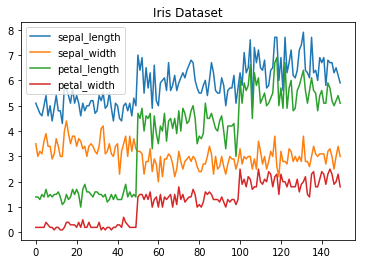
\includegraphics[width=0.7\textwidth]{Images/matplotlib_line_chart-min.png}
    \caption{Line Chart Example}
    \label{fig1}
\end{figure}

\textbf{Histograms} \\
The graphic representation of data points arranged into user-specified ranges is called a histogram. The histogram, which resembles a bar graph in appearance, condenses a data series into an intuitive visual by taking numerous data points and organising them into logical ranges or bins.

\begin{figure}[H]
    \centering
    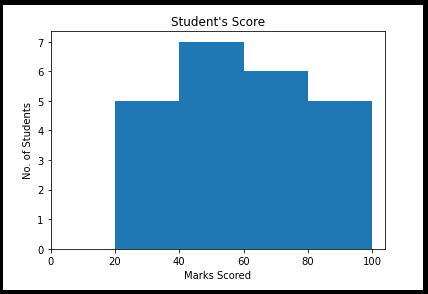
\includegraphics[width=0.7\textwidth]{Images/45209histo.png}
    \caption{Histograms Example}
    \label{fig1}
\end{figure}


Characteristics Of Histogram:
\begin{itemize}
    \item The Histogram is used to get any unusual observations in the give en dataset.
\item Measured on an interval scale of given numerical values with several data bins.
\item The Y-axis represents the number of \% of occurrences in the data
\item The X-axis represents data distributions.
\end{itemize}

\textbf{Scatter plots} \\
Data points are plotted across both axes (horizontal and vertical) in scatter plots to show how each axis is associated with the other. Generally, we should examine how dependent and independent are aligned before the EDA process and frequently during Data Science/Machine Learning deployment. It could be positive, negative, or occasionally dispersed over the graph.

\begin{figure}[H]
    \centering
    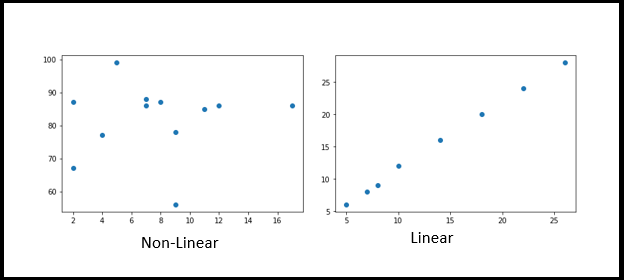
\includegraphics[width=0.7\textwidth]{Images/53461Scatter plots.png}
    \caption{Scatter Plot Example}
    \label{fig1}
\end{figure}
